\documentclass{article}

\usepackage{graphicx}
\usepackage{booktabs}
\usepackage{tabularx}
\usepackage{hyperref}
\usepackage{color}

\title{SE 3XA3: User Guide\\GrateBox}

\author{Team 8, Grate
		\\ Kelvin Lin (linkk4)
		\\ Eric Chaput (chaputem)
		\\ Jin Liu (liu456)
}

\date{}

%% Comments

\usepackage{color}

\newif\ifcomments\commentstrue

\ifcomments
\newcommand{\authornote}[3]{\textcolor{#1}{[#3 ---#2]}}
\newcommand{\todo}[1]{\textcolor{red}{[TODO: #1]}}
\else
\newcommand{\authornote}[3]{}
\newcommand{\todo}[1]{}
\fi

\newcommand{\wss}[1]{\authornote{blue}{SS}{#1}}
\newcommand{\ds}[1]{\authornote{red}{DS}{#1}}
\newcommand{\mj}[1]{\authornote{red}{MSN}{#1}}
\newcommand{\cm}[1]{\authornote{red}{CM}{#1}}
\newcommand{\mh}[1]{\authornote{red}{MH}{#1}}

% team members should be added for each team, like the following
% all comments left by the TAs or the instructor should be addressed
% by a corresponding comment from the Team

\newcommand{\tm}[1]{\authornote{magenta}{Team}{#1}}


\begin{document}

\newpage

\maketitle

\section{How to access GrateBox}

GrateBox is a web application created to educate and entertain users by the use 
of genetic algorithms. There are two ways to access and use the GrateBox 
application. The first method iss to navigate to the the url to access the 
online version of GrateBox. To do so, open your internet browser and enter the 
following url 
\href{http://ugweb.cas.mcmaster.ca/~linkk4/}{http://ugweb.cas.mcmaster.ca/~linkk4/}. 
GrateBox can also be run locally on your machine. To do this first navigate to 
to GrateBox's GitHub repository found at the following url 
\href{https://gitlab.cas.mcmaster.ca/linkk4/GrateBox/tree/master}{https://gitlab.cas.mcmaster.ca/linkk4/GrateBox/tree/master}. 
Then install the zip file by clicking the install button near the top right of 
the screen to download the zip file containing GrateBox. Extract the zip file to 
a location of your choosing and navigate to the src folder and double select the 
GrateBoxBootStrap.html file to open it.

\section {How to use Gratebox}

Once you access GrateBox, you will see a number of things All of GrateBox's 
functionality is contained on one screen. Under the simulation title, you will 
see a simulation of a randomly created generation of cars. By default, this 
simulation will generate an initial population of three cars for the first 
generation, with the best two cars of each generation selected for breeding the 
next generation, and a mutation rate of two percent. These values can be seen 
under the Parameters title, and can be edited by the user. To edit a parameter, 
simply enter a new value under the corresponding parameter title and click 
enter. The simulation will then be run from the start with the new values. Also 
under the Parameters title can be seen a pause button. To pause the simulation 
at any time click the pause button. To unpause the simulation, simply select the 
pause button again. Further down the page you will see text giving you 
information about the simulation and about GrateBox and Genetic Algorithms in 
general.

\begin{figure}
  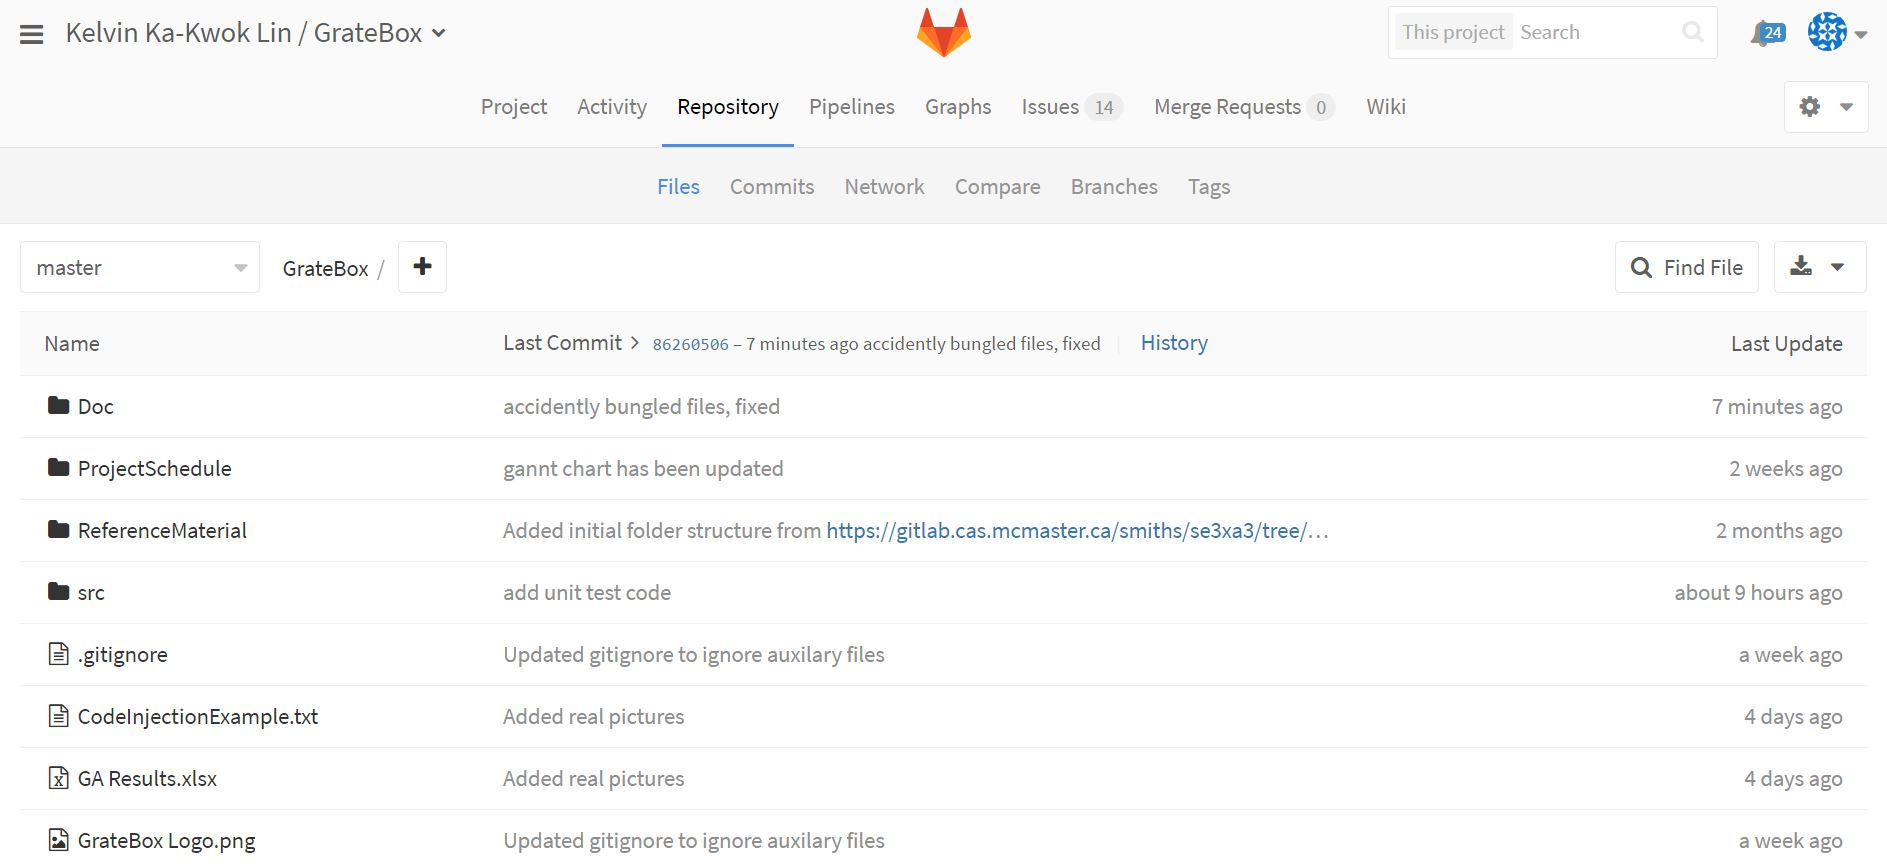
\includegraphics[width=\linewidth]{Images/GrateBoxGitRep.JPG}
  \caption{The view of the GrateBox repository on GitHub. You can see the 
download button in the top right next to the Find File button.}
  \label{fig:GitRep1}
\end{figure}

\begin{figure}
  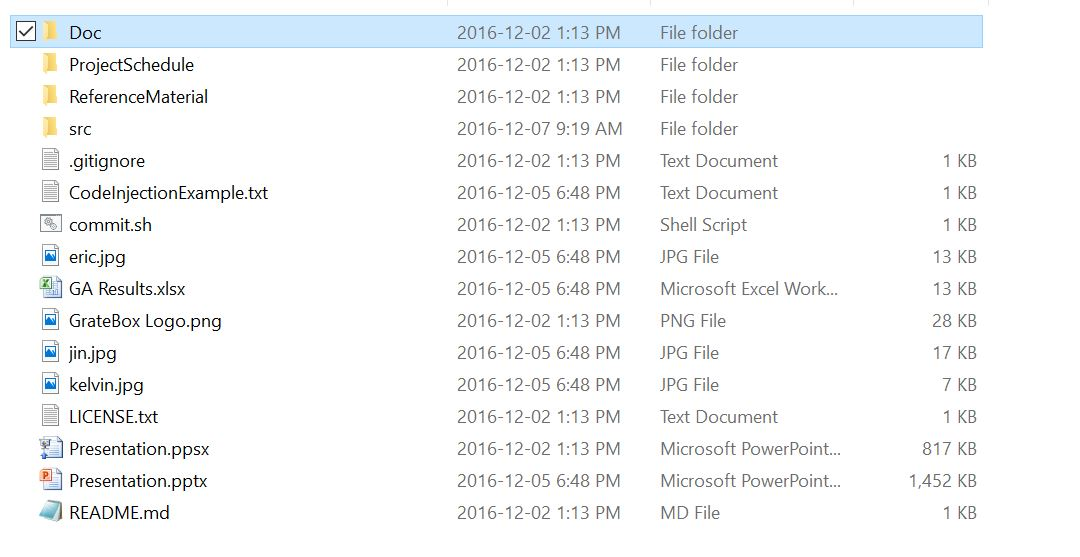
\includegraphics[width=\linewidth]{Images/GrateBoxGitRep2.JPG}
  \caption{The contents of the GrateBox repository. The src folder can be seen 
clearly as the forth from the top.}
  \label{fig:GitRep2}
\end{figure}

\begin{figure}
  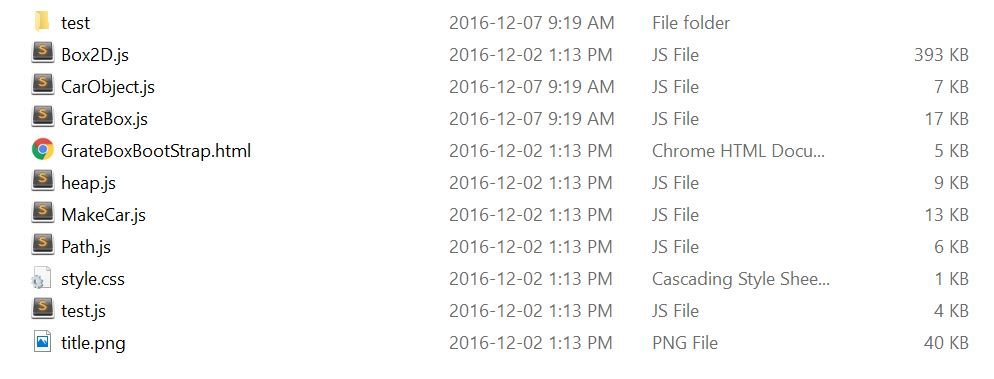
\includegraphics[width=\linewidth]{Images/GrateBoxGitRep3.JPG}
  \caption{The contents of the src folder. Open the GrateBoxBootStrap html file 
to access GrateBox.}
  \label{fig:GitRep3}
\end{figure}

\begin{figure}
  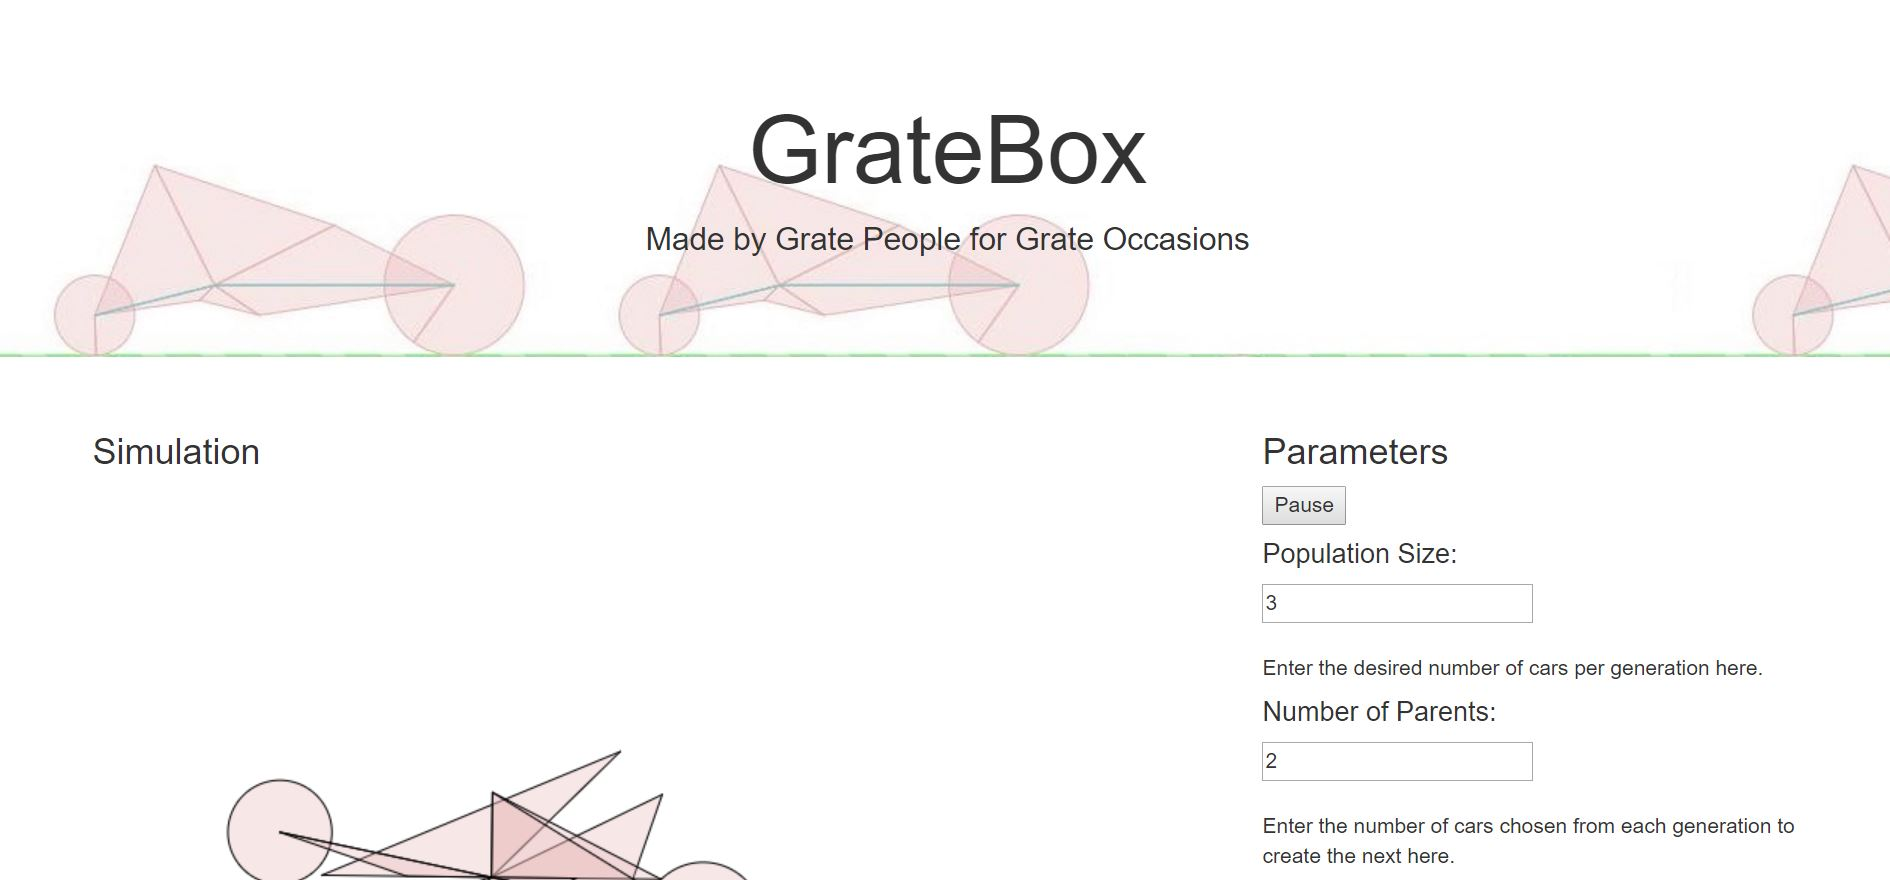
\includegraphics[width=\linewidth]{Images/GrateBoxFirstScreen.JPG}
  \caption{The initial view of GrateBox.}
  \label{fig:First1}
\end{figure}

\begin{figure}
  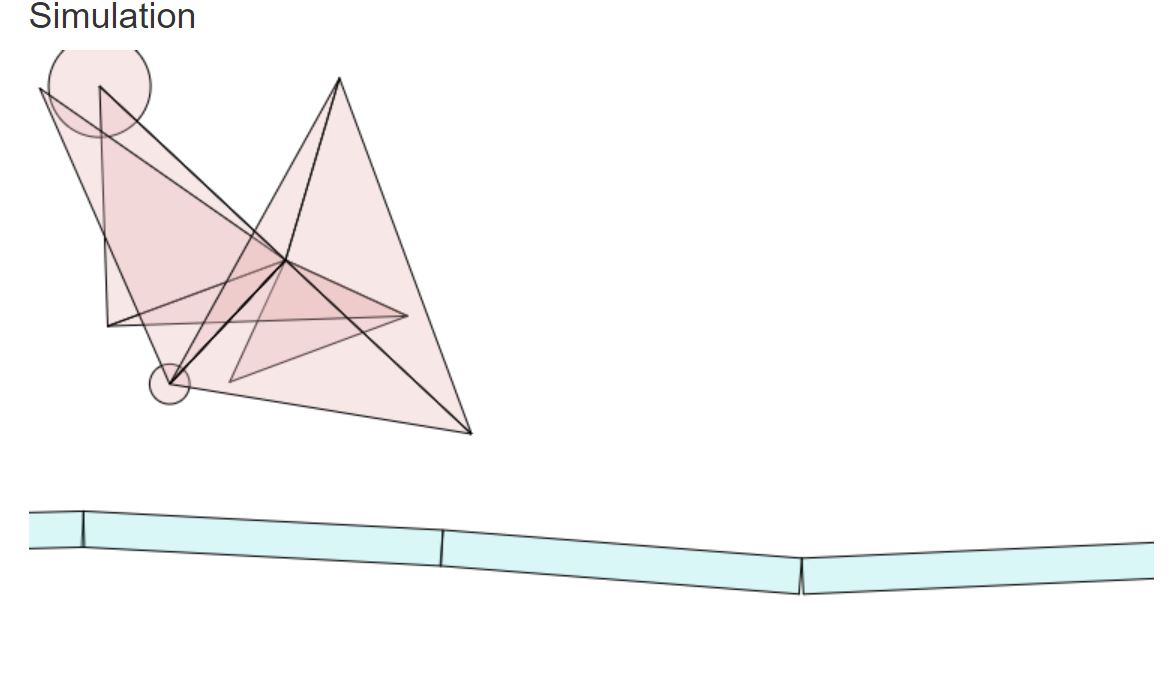
\includegraphics[width=\linewidth]{Images/GrateBoxSimulation.JPG}
  \caption{The simulation display.}
  \label{fig:Sim1}
\end{figure}

\begin{figure}
  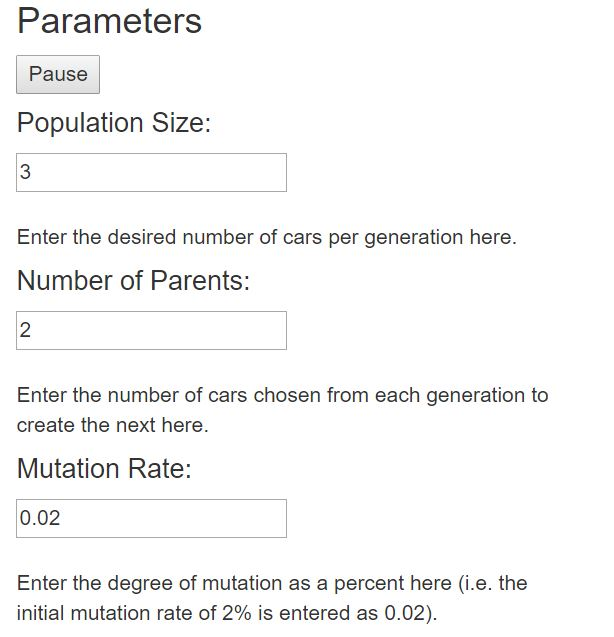
\includegraphics[width=\linewidth]{Images/GrateBoxParameters.JPG}
  \caption{The parameters display.}
  \label{fig:Param1}
\end{figure}

\begin{figure}
  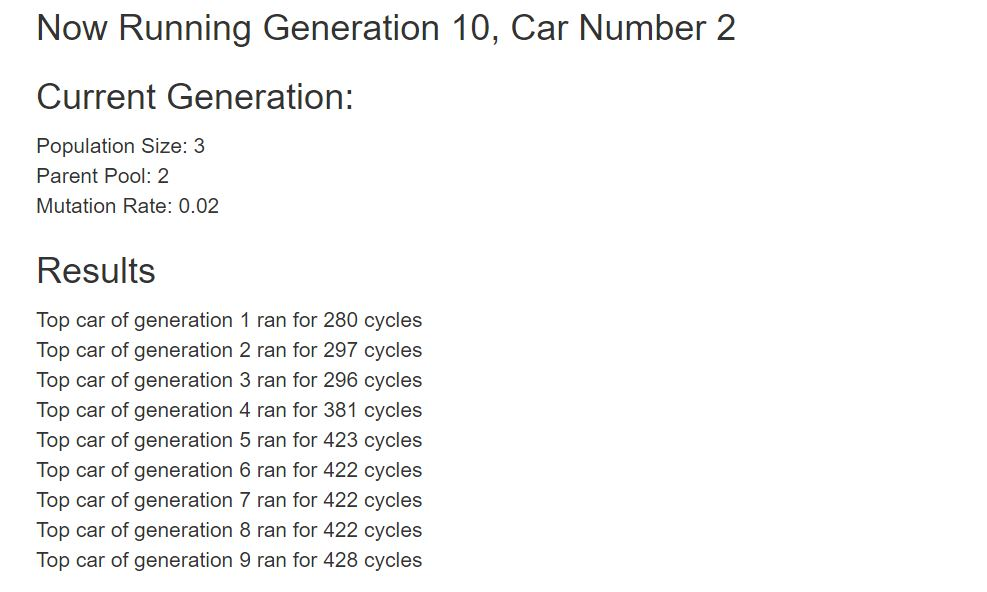
\includegraphics[width=\linewidth]{Images/GrateBoxSimulationInfo.JPG}
  \caption{The info at the bottom of the screen showing simulation results.}
  \label{fig:Info1}
\end{figure}

\begin{figure}
  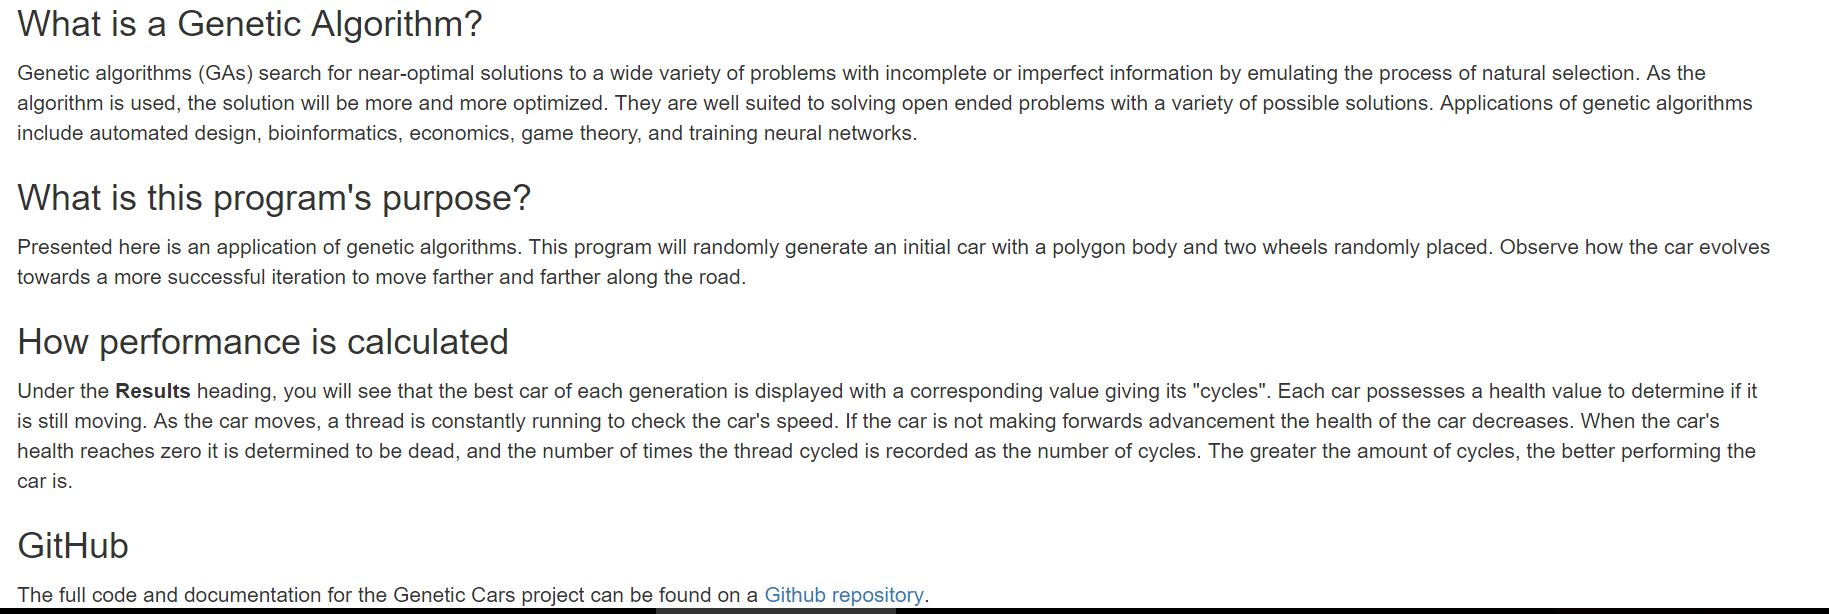
\includegraphics[width=\linewidth]{Images/GrateBoxInfo.JPG}
  \caption{The info at the bottom of the screen describing GrateBox and Genetic 
Algorithms.}
  \label{fig:Info2}
\end{figure}

\end{document}

